%------------------------------------------------------------------------------
\chapter{Challenges with segment selection algorithm for new triggers} 
\label{sec:app_3}
%------------------------------------------------------------------------------
\begin{figure}[t!]
\centering
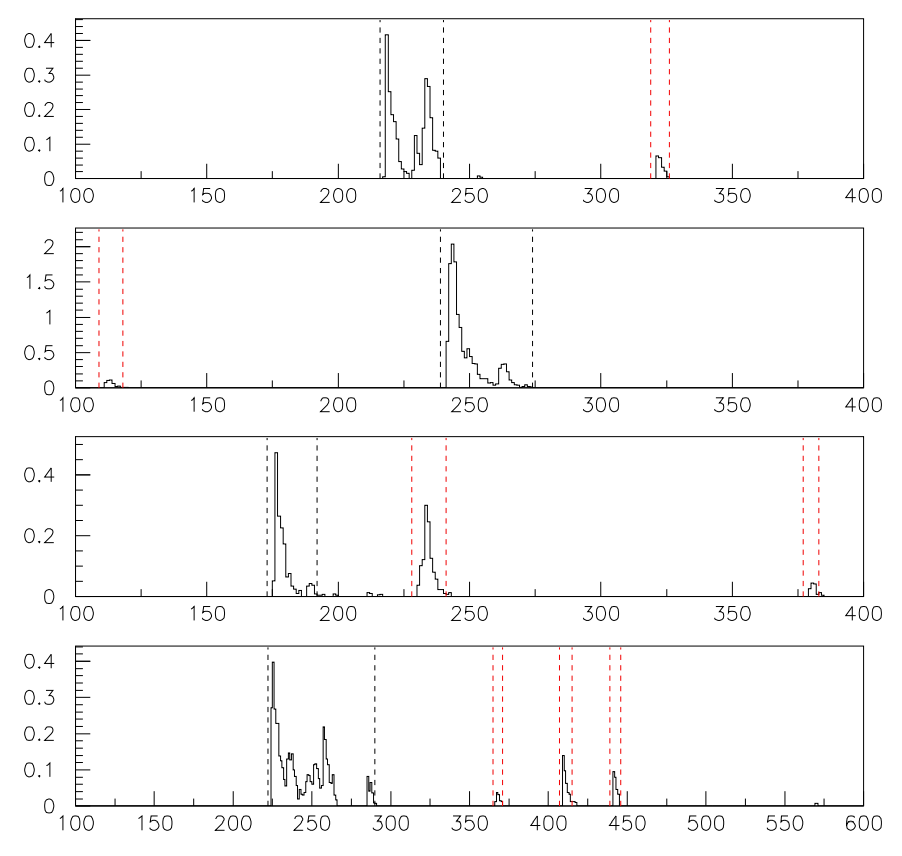
\includegraphics[width=0.75\textwidth]{thesis_figures/App3/Segment_selection.png}
\caption{Examples of the segment selection process applied on FADC traces. The main segment is enclosed within black lines. The red lines enclose the secondary segments found by the algorithm. Only the black segment is used for top-down selection. The x-scale is in VEM units and the y-axis denotes time in ns. Taken from~\cite{gap_segment_selection}.}
\label{fig:segment_selection}
\end{figure}

This appendix aims to present some interesting reconstructed events that were observed in the background training sample when new triggers were used for the neutrino analysis. As mentioned before in sec.~\ref{subsec:reco_presel} and described in more detail in~\cite{gap_top_down_module} a segment selection process is applied to improve the quality of angular reconstruction. A small example of the working of the process is shown in Fig.~\ref{fig:segment_selection}. It was observed while performing the neutrino analysis with new triggers some events were mis-reconstructed due to an untuned segment selection algorithm. These events were further checked and reconstructed using the standard reconstruction used for inclined UHECRs at the Pierre Auger Observatory which classified most of these as noise. It was also noticed that the problems with the segment selection algorithm for the new triggers could primarily arise from the presence of multiple peaks with similar amplitudes in the waveform. There is also an argument that the primary purpose of the segment selection algorithm i.e. the reduction of accidental muons which change the start time of the signal might already be addressed with the design of the new triggers thus decreasing the overall need for such an algorithm. However, these are only hypothesis and need to be confirmed with further studies. Thus, due to the inability to confirm the validity of the segment selection process for the new triggers, the algorithm was not applied to stations with these triggers in a way that the reconstruction for stations with old triggers remained unaffected. Some pictures of events which were investigated are shown below. The pictures are taken from the GUI display available to look at events within the collaboration.

Fig.~\ref{fig:bad_segment_selection} shows an event where the segmentation algorithm failed to find the correct segment for the station with the MoPS trigger. 

As mentioned before in Outlook a properly tuned segmentation algorithm could also help the neutrino search with new triggers. Fig.~\ref{fig:good_segment_selection} shows an event where the MoPS signal is selected with a start time of 200ns but is out of time with other stations with start times close to 240ns. A segment selection algorithm could help in this case to select the correct segment for the station with MoPS trigger.

Fig.~\ref{fig:bad_ang_fit} shows an example of an event with a bad angular fit. The indication of the bad quality can only be gauged via the $\chi^2_{\text{red}}$ and does not show up in the error on zenith angle. Such events though small in number are essential to be excluded from the analysis to avoid any bias in the final result. This is done with the Angular fit quality cut described before. 

The event shown in Fig.~\ref{fig:bad_fisher} shows an example of an event which had an evaluated Fisher value close to the cut value. The event had no peculiar feature which could classify it as a neutrino or otherwise.

\begin{figure}[h!]
  \centering
  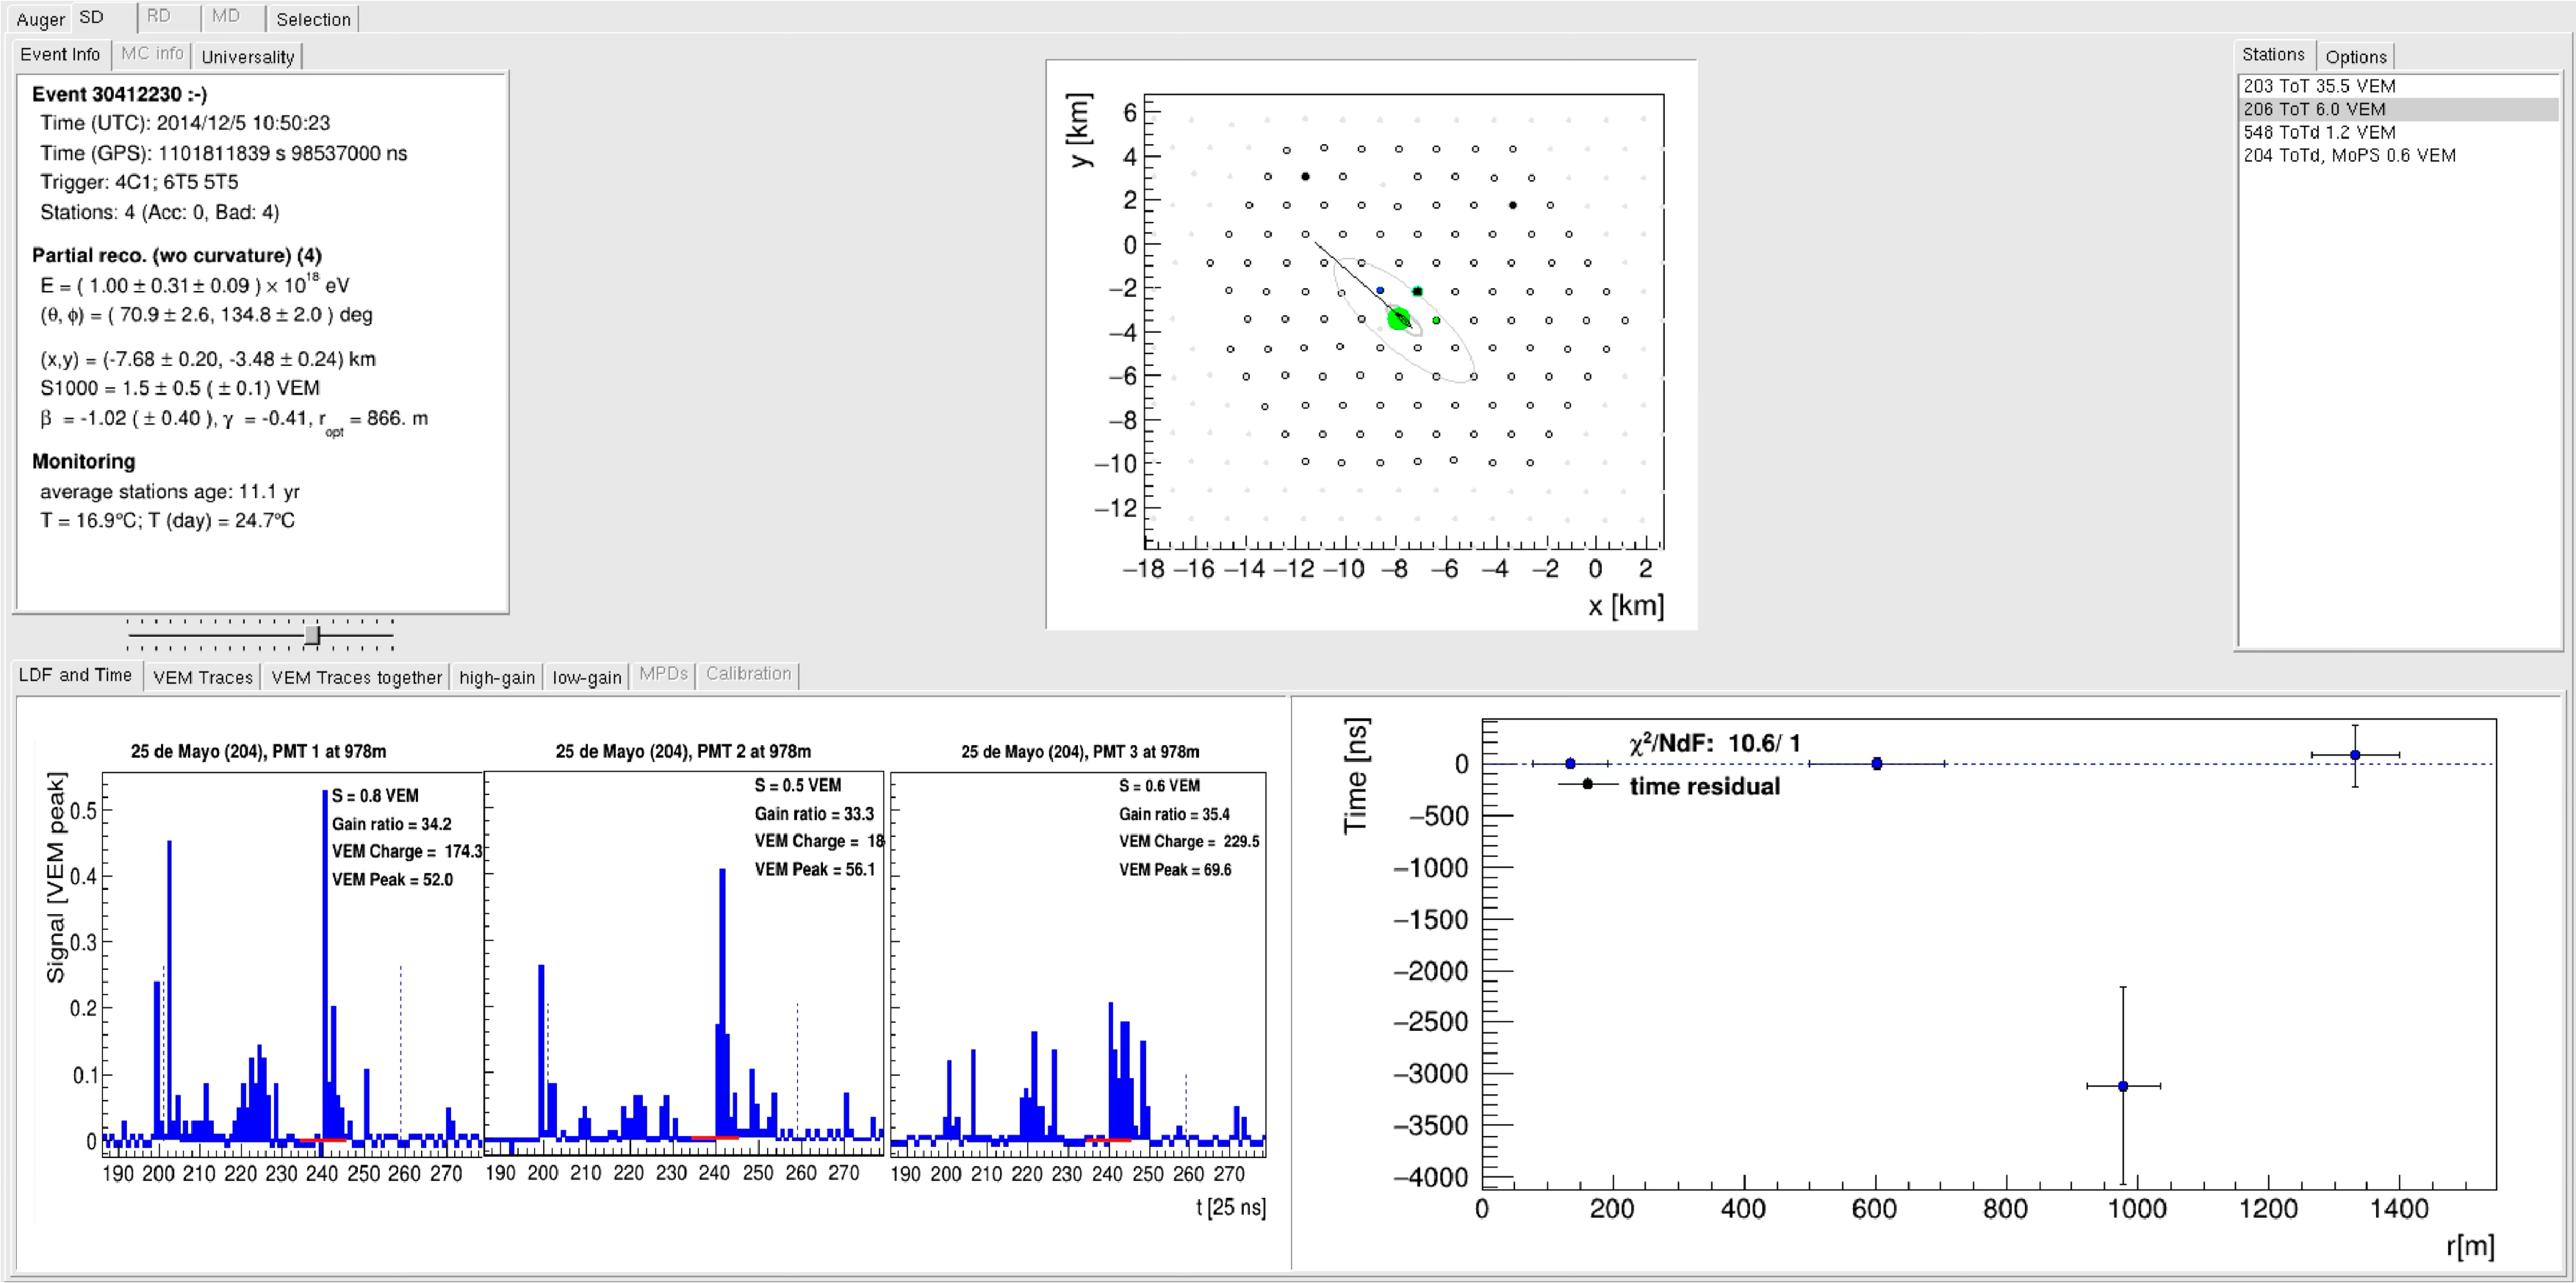
\includegraphics[width=\textwidth]{thesis_figures/App3/Bad_segment.pdf}
  \caption{An example of an event where segment selection did on a station with the MOPS trigger. Due to the two similar peaks seen in MoPS trace for the station 204, the segment selection algorithm could not find the correct segment and led to a mis-reconstruction of zenith angle.}
  \label{fig:bad_segment_selection}
  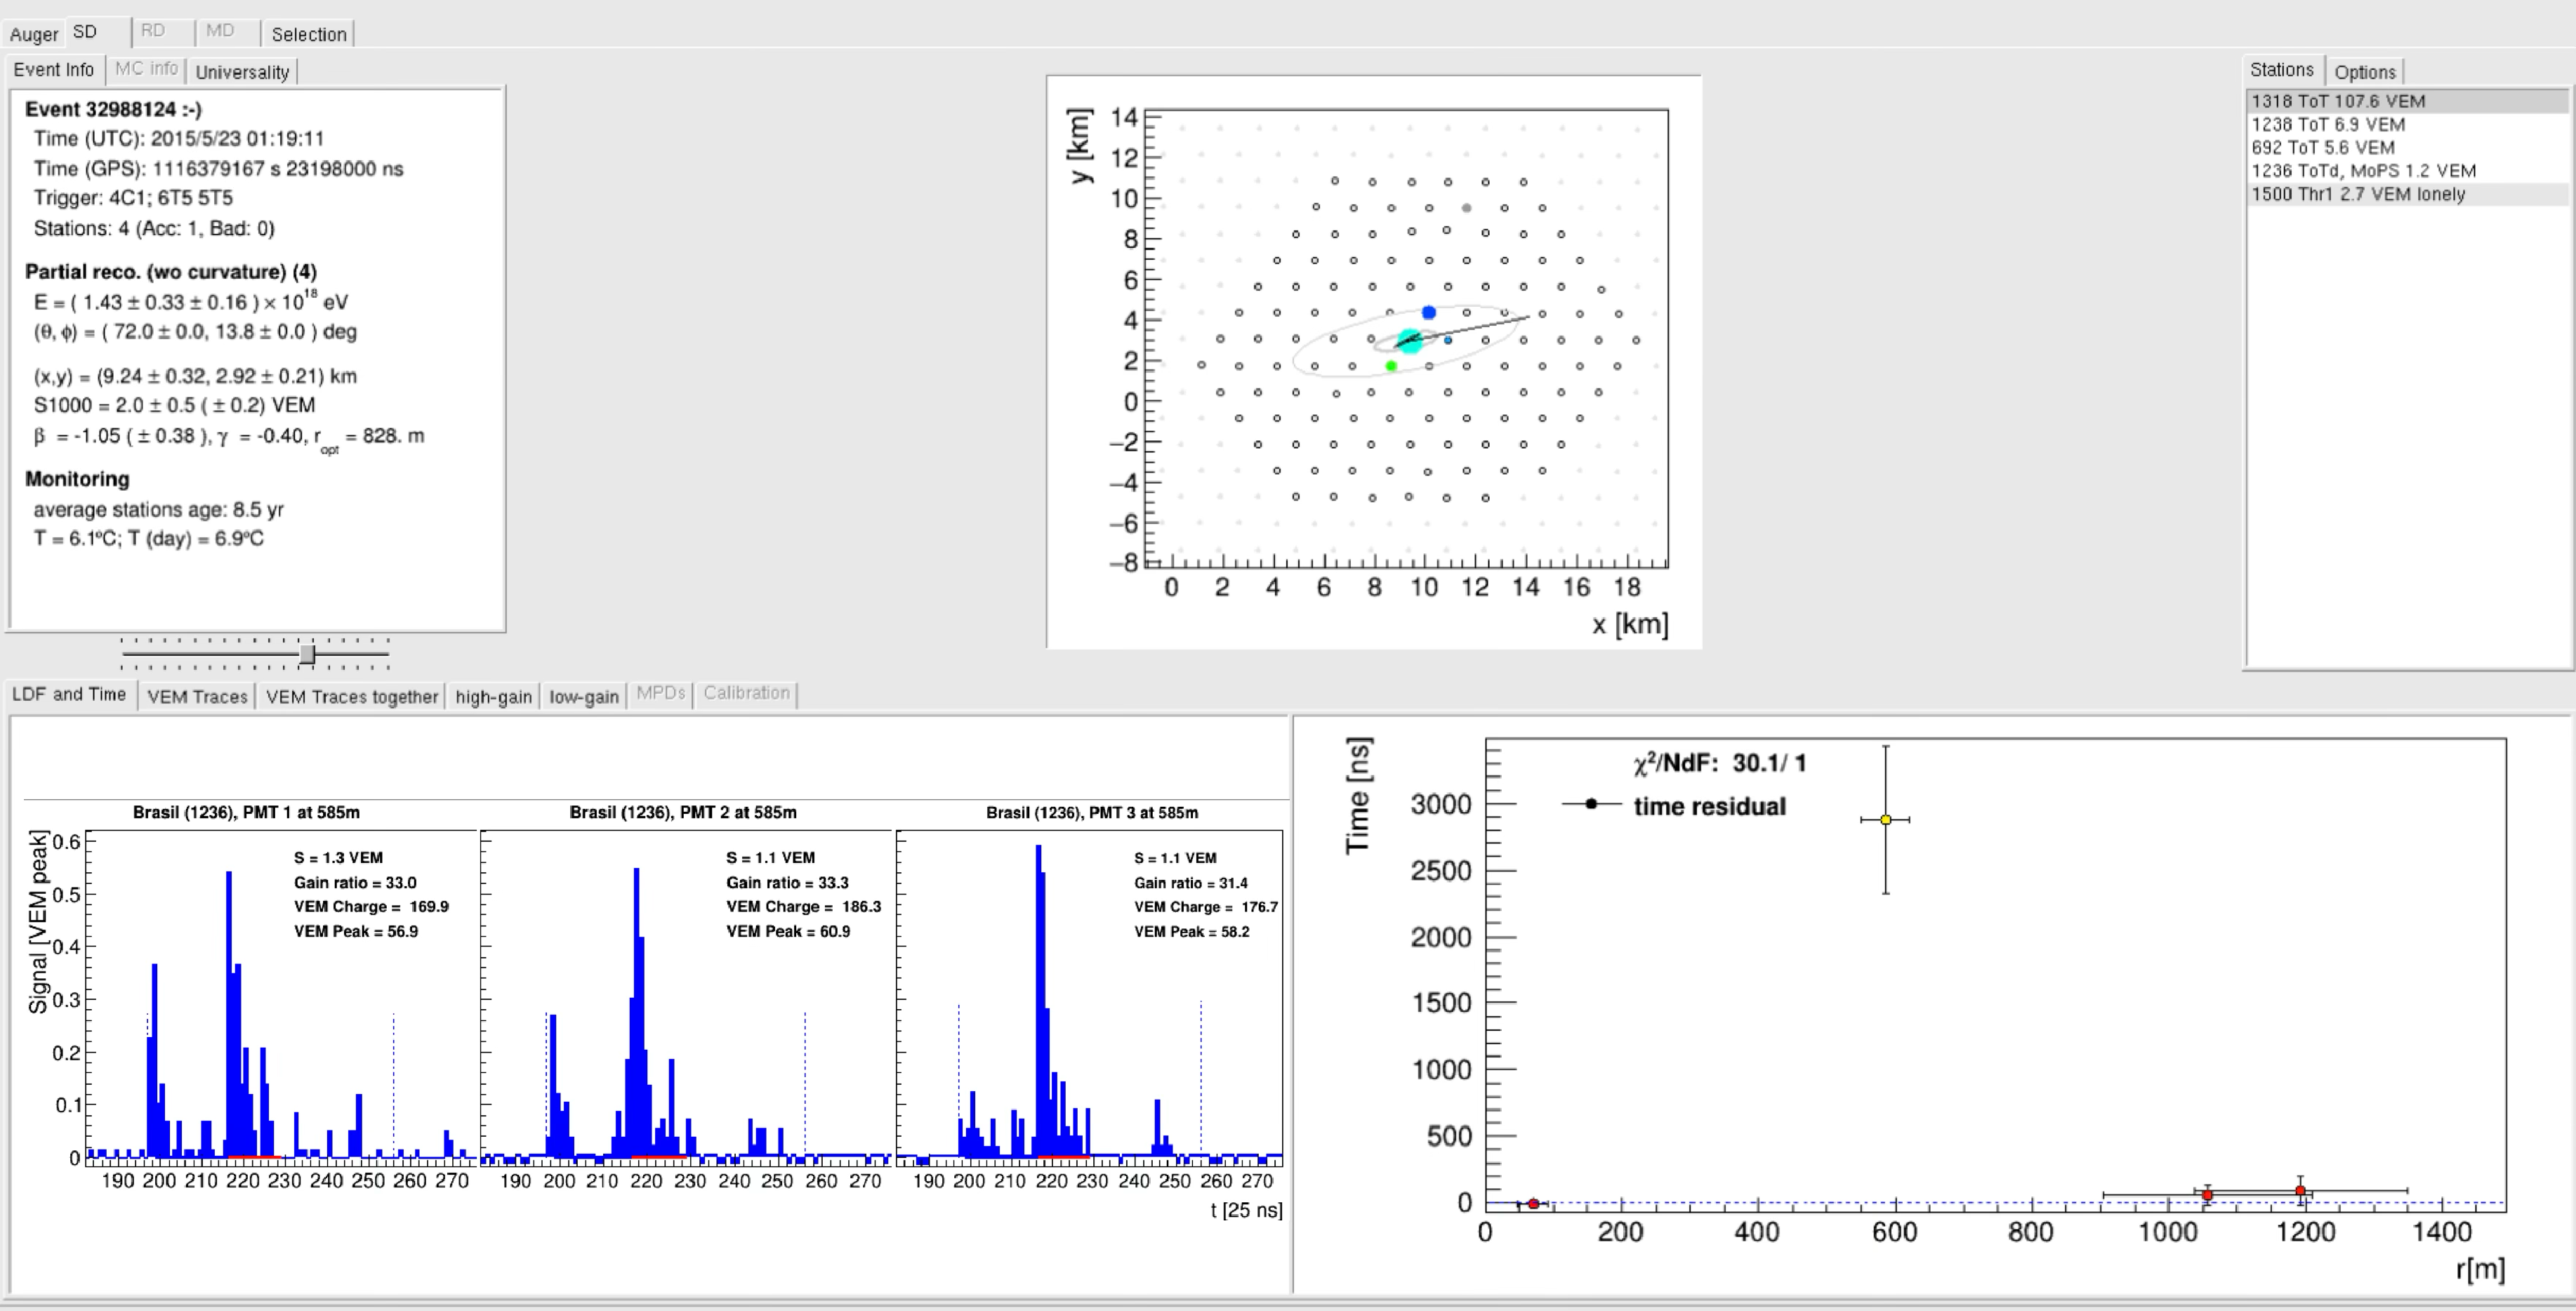
\includegraphics[width=\textwidth]{thesis_figures/App3/MoPS_peak_selection.pdf}
  \caption{An example of an event where segment selection could help in the reconstruction. The MoPS signal is selected with a start time of 200ns but is out of time with other stations (240ns). A segment selection algorithm could help in this case to select the correct segment for the station with MoPS trigger.}
  \label{fig:good_segment_selection}

\end{figure}

\begin{figure}[h!]
  \centering
  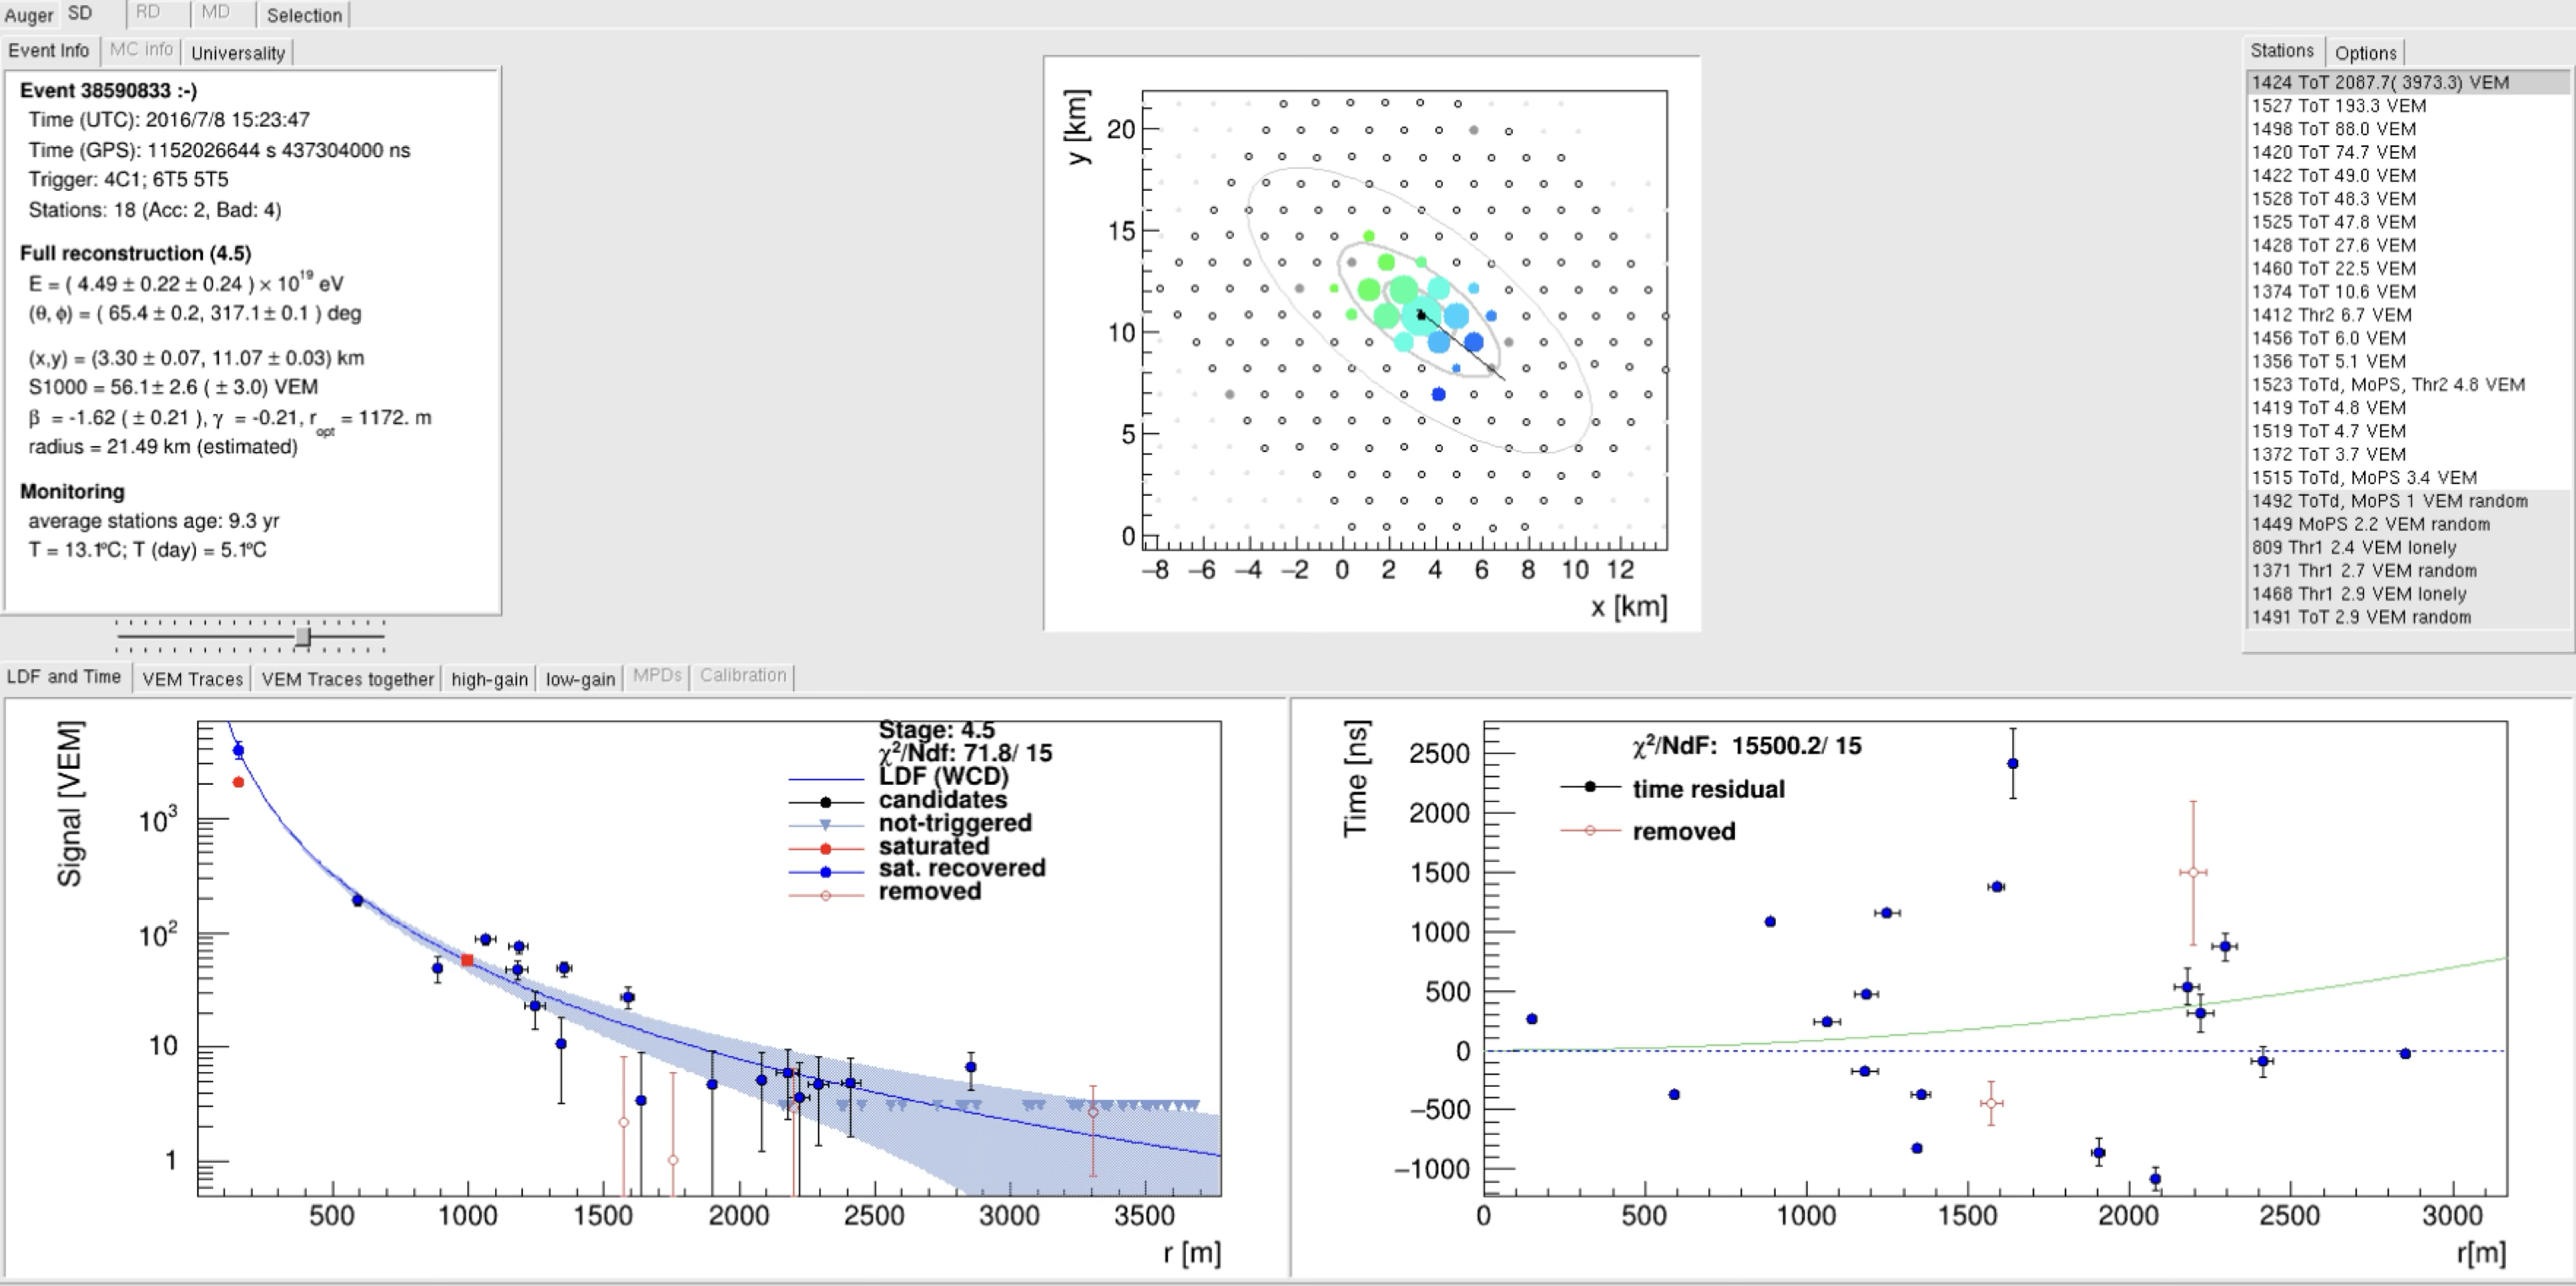
\includegraphics[width=\textwidth]{thesis_figures/App3/bad_ang_fit.png}
  \caption{Example of an event with a bad angular fit. The indication of the bad quality can only be gauged via the $\chi^2_{red}$.}
  \label{fig:bad_ang_fit}
  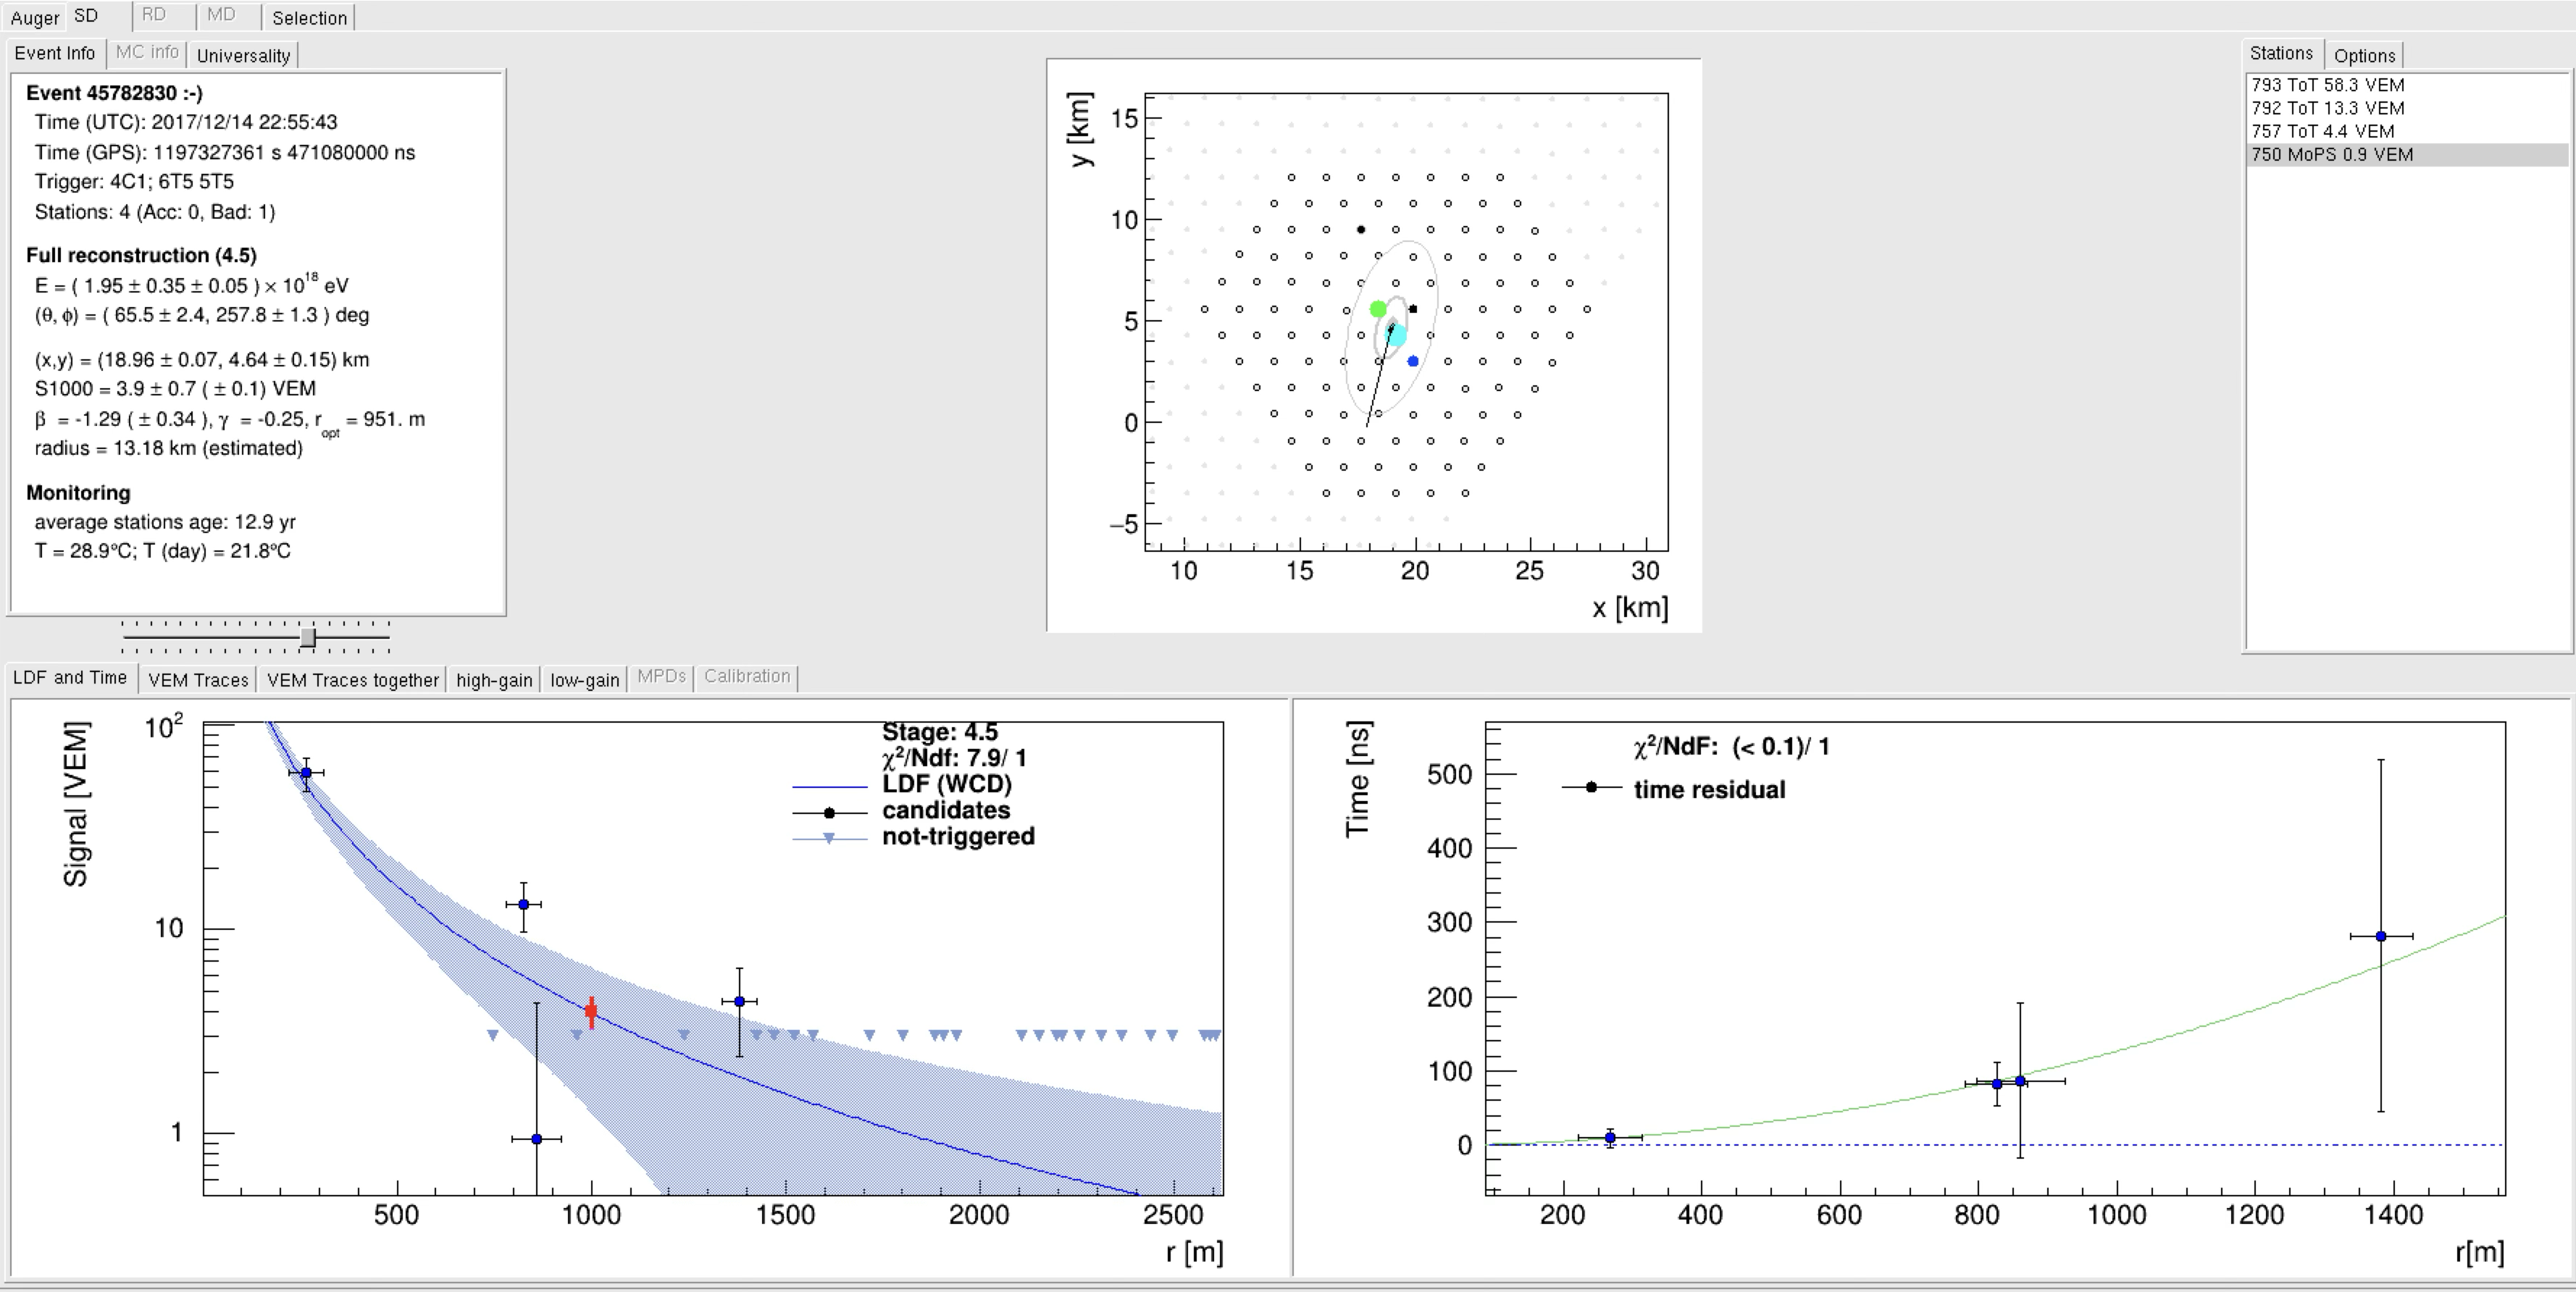
\includegraphics[width=\textwidth]{thesis_figures/App3/Bkg_close_noproblem.png}
  \caption{An example of an event which had an evaluated Fisher value close to the cut value. No particular feature was found for this event which classified it as a neutrino like event or otherwise.} 
  \label{fig:bad_fisher}

\end{figure}
